% Created by tikzDevice version 0.8.1 on 2015-11-15 18:06:42
% !TEX encoding = UTF-8 Unicode
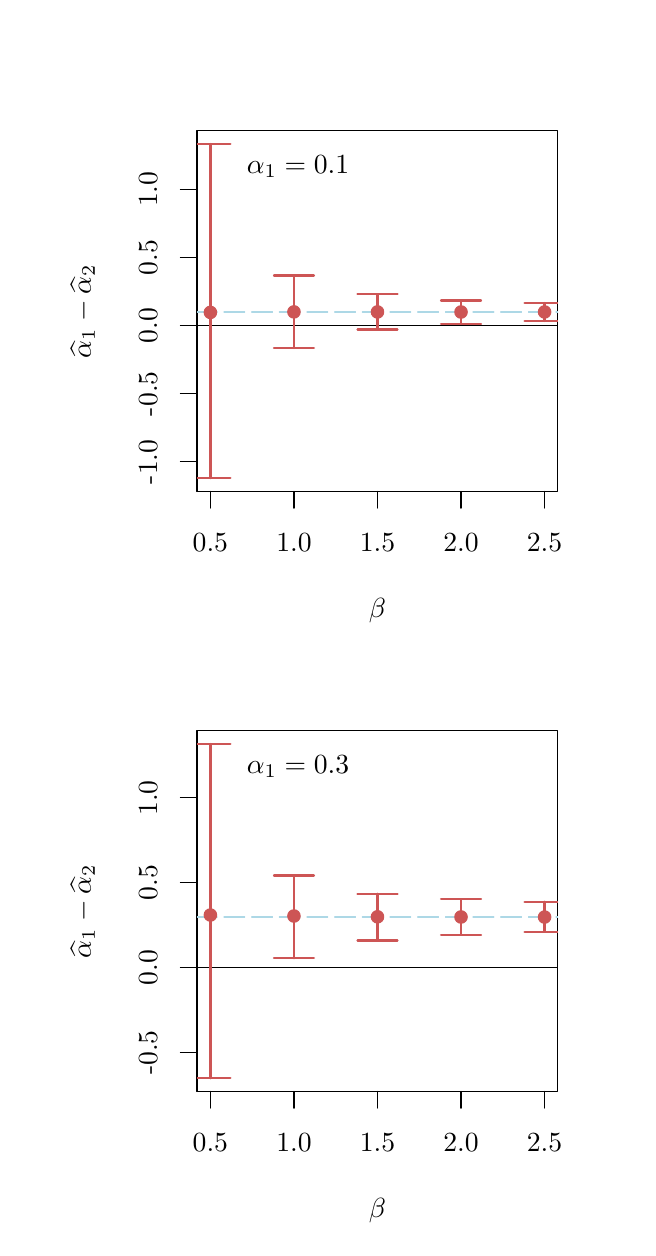
\begin{tikzpicture}[x=1pt,y=1pt]
\definecolor{fillColor}{RGB}{255,255,255}
\path[use as bounding box,fill=fillColor,fill opacity=0.00] (0,0) rectangle (216.81,433.62);
\begin{scope}
\path[clip] ( 61.20,266.01) rectangle (191.61,396.42);
\definecolor{drawColor}{RGB}{255,255,255}
\definecolor{fillColor}{RGB}{255,255,255}

\path[draw=drawColor,line width= 0.4pt,line join=round,line cap=round,fill=fillColor] ( 66.03,330.73) circle (  2.25);

\path[draw=drawColor,line width= 0.4pt,line join=round,line cap=round,fill=fillColor] ( 96.22,330.91) circle (  2.25);

\path[draw=drawColor,line width= 0.4pt,line join=round,line cap=round,fill=fillColor] (126.40,330.90) circle (  2.25);

\path[draw=drawColor,line width= 0.4pt,line join=round,line cap=round,fill=fillColor] (156.59,330.87) circle (  2.25);

\path[draw=drawColor,line width= 0.4pt,line join=round,line cap=round,fill=fillColor] (186.78,330.89) circle (  2.25);
\end{scope}
\begin{scope}
\path[clip] (  0.00,  0.00) rectangle (216.81,433.62);
\definecolor{drawColor}{RGB}{0,0,0}

\path[draw=drawColor,line width= 0.4pt,line join=round,line cap=round] ( 66.03,266.01) -- (186.78,266.01);

\path[draw=drawColor,line width= 0.4pt,line join=round,line cap=round] ( 66.03,266.01) -- ( 66.03,260.01);

\path[draw=drawColor,line width= 0.4pt,line join=round,line cap=round] ( 96.22,266.01) -- ( 96.22,260.01);

\path[draw=drawColor,line width= 0.4pt,line join=round,line cap=round] (126.40,266.01) -- (126.40,260.01);

\path[draw=drawColor,line width= 0.4pt,line join=round,line cap=round] (156.59,266.01) -- (156.59,260.01);

\path[draw=drawColor,line width= 0.4pt,line join=round,line cap=round] (186.78,266.01) -- (186.78,260.01);

\node[text=drawColor,anchor=base,inner sep=0pt, outer sep=0pt, scale=  1.00] at ( 66.03,244.41) {0.5};

\node[text=drawColor,anchor=base,inner sep=0pt, outer sep=0pt, scale=  1.00] at ( 96.22,244.41) {1.0};

\node[text=drawColor,anchor=base,inner sep=0pt, outer sep=0pt, scale=  1.00] at (126.40,244.41) {1.5};

\node[text=drawColor,anchor=base,inner sep=0pt, outer sep=0pt, scale=  1.00] at (156.59,244.41) {2.0};

\node[text=drawColor,anchor=base,inner sep=0pt, outer sep=0pt, scale=  1.00] at (186.78,244.41) {2.5};

\path[draw=drawColor,line width= 0.4pt,line join=round,line cap=round] ( 61.20,276.72) -- ( 61.20,375.22);

\path[draw=drawColor,line width= 0.4pt,line join=round,line cap=round] ( 61.20,276.72) -- ( 55.20,276.72);

\path[draw=drawColor,line width= 0.4pt,line join=round,line cap=round] ( 61.20,301.34) -- ( 55.20,301.34);

\path[draw=drawColor,line width= 0.4pt,line join=round,line cap=round] ( 61.20,325.97) -- ( 55.20,325.97);

\path[draw=drawColor,line width= 0.4pt,line join=round,line cap=round] ( 61.20,350.59) -- ( 55.20,350.59);

\path[draw=drawColor,line width= 0.4pt,line join=round,line cap=round] ( 61.20,375.22) -- ( 55.20,375.22);

\node[text=drawColor,rotate= 90.00,anchor=base,inner sep=0pt, outer sep=0pt, scale=  1.00] at ( 46.80,276.72) {-1.0};

\node[text=drawColor,rotate= 90.00,anchor=base,inner sep=0pt, outer sep=0pt, scale=  1.00] at ( 46.80,301.34) {-0.5};

\node[text=drawColor,rotate= 90.00,anchor=base,inner sep=0pt, outer sep=0pt, scale=  1.00] at ( 46.80,325.97) {0.0};

\node[text=drawColor,rotate= 90.00,anchor=base,inner sep=0pt, outer sep=0pt, scale=  1.00] at ( 46.80,350.59) {0.5};

\node[text=drawColor,rotate= 90.00,anchor=base,inner sep=0pt, outer sep=0pt, scale=  1.00] at ( 46.80,375.22) {1.0};

\path[draw=drawColor,line width= 0.4pt,line join=round,line cap=round] ( 61.20,266.01) --
	(191.61,266.01) --
	(191.61,396.42) --
	( 61.20,396.42) --
	( 61.20,266.01);
\end{scope}
\begin{scope}
\path[clip] (  0.00,216.81) rectangle (216.81,433.62);
\definecolor{drawColor}{RGB}{0,0,0}

\node[text=drawColor,anchor=base,inner sep=0pt, outer sep=0pt, scale=  1.00] at (126.41,220.41) {$\beta$};

\node[text=drawColor,rotate= 90.00,anchor=base,inner sep=0pt, outer sep=0pt, scale=  1.00] at ( 22.80,331.22) {$\widehat{\alpha}_1 - \widehat{\alpha}_2$};
\end{scope}
\begin{scope}
\path[clip] ( 61.20,266.01) rectangle (191.61,396.42);
\definecolor{drawColor}{RGB}{0,0,0}

\node[text=drawColor,anchor=base west,inner sep=0pt, outer sep=0pt, scale=  1.00] at ( 79.20,380.98) {$\alpha_1=0.1$};
\definecolor{drawColor}{RGB}{173,216,230}

\path[draw=drawColor,line width= 0.8pt,dash pattern=on 7pt off 3pt ,line join=round,line cap=round] ( 61.20,330.89) -- (191.61,330.89);

\path[draw=drawColor,line width= 0.8pt,dash pattern=on 7pt off 3pt ,line join=round,line cap=round] ( 61.20,330.89) -- (191.61,330.89);

\path[draw=drawColor,line width= 0.8pt,dash pattern=on 7pt off 3pt ,line join=round,line cap=round] ( 61.20,330.89) -- (191.61,330.89);

\path[draw=drawColor,line width= 0.8pt,dash pattern=on 7pt off 3pt ,line join=round,line cap=round] ( 61.20,330.89) -- (191.61,330.89);

\path[draw=drawColor,line width= 0.8pt,dash pattern=on 7pt off 3pt ,line join=round,line cap=round] ( 61.20,330.89) -- (191.61,330.89);
\definecolor{drawColor}{RGB}{0,0,0}

\path[draw=drawColor,line width= 0.4pt,line join=round,line cap=round] ( 61.20,325.97) -- (191.61,325.97);
\definecolor{drawColor}{RGB}{205,85,85}

\path[draw=drawColor,line width= 0.8pt,line join=round,line cap=round] ( 66.03,270.84) -- ( 66.03,391.59);

\path[draw=drawColor,line width= 0.8pt,line join=round,line cap=round] ( 58.80,270.84) --
	( 66.03,270.84) --
	( 73.26,270.84);

\path[draw=drawColor,line width= 0.8pt,line join=round,line cap=round] ( 73.26,391.59) --
	( 66.03,391.59) --
	( 58.80,391.59);

\path[draw=drawColor,line width= 0.8pt,line join=round,line cap=round] ( 96.22,317.85) -- ( 96.22,344.08);

\path[draw=drawColor,line width= 0.8pt,line join=round,line cap=round] ( 88.99,317.85) --
	( 96.22,317.85) --
	(103.44,317.85);

\path[draw=drawColor,line width= 0.8pt,line join=round,line cap=round] (103.44,344.08) --
	( 96.22,344.08) --
	( 88.99,344.08);

\path[draw=drawColor,line width= 0.8pt,line join=round,line cap=round] (126.40,324.52) -- (126.40,337.30);

\path[draw=drawColor,line width= 0.8pt,line join=round,line cap=round] (119.18,324.52) --
	(126.40,324.52) --
	(133.63,324.52);

\path[draw=drawColor,line width= 0.8pt,line join=round,line cap=round] (133.63,337.30) --
	(126.40,337.30) --
	(119.18,337.30);

\path[draw=drawColor,line width= 0.8pt,line join=round,line cap=round] (156.59,326.65) -- (156.59,335.06);

\path[draw=drawColor,line width= 0.8pt,line join=round,line cap=round] (149.37,326.65) --
	(156.59,326.65) --
	(163.82,326.65);

\path[draw=drawColor,line width= 0.8pt,line join=round,line cap=round] (163.82,335.06) --
	(156.59,335.06) --
	(149.37,335.06);

\path[draw=drawColor,line width= 0.8pt,line join=round,line cap=round] (186.78,327.61) -- (186.78,334.14);

\path[draw=drawColor,line width= 0.8pt,line join=round,line cap=round] (179.55,327.61) --
	(186.78,327.61) --
	(194.01,327.61);

\path[draw=drawColor,line width= 0.8pt,line join=round,line cap=round] (194.01,334.14) --
	(186.78,334.14) --
	(179.55,334.14);
\definecolor{fillColor}{RGB}{205,85,85}

\path[draw=drawColor,line width= 0.4pt,line join=round,line cap=round,fill=fillColor] ( 66.03,330.73) circle (  2.25);

\path[draw=drawColor,line width= 0.4pt,line join=round,line cap=round,fill=fillColor] ( 96.22,330.91) circle (  2.25);

\path[draw=drawColor,line width= 0.4pt,line join=round,line cap=round,fill=fillColor] (126.40,330.90) circle (  2.25);

\path[draw=drawColor,line width= 0.4pt,line join=round,line cap=round,fill=fillColor] (156.59,330.87) circle (  2.25);

\path[draw=drawColor,line width= 0.4pt,line join=round,line cap=round,fill=fillColor] (186.78,330.89) circle (  2.25);
\end{scope}
\begin{scope}
\path[clip] ( 61.20, 49.20) rectangle (191.61,179.61);
\definecolor{drawColor}{RGB}{255,255,255}
\definecolor{fillColor}{RGB}{255,255,255}

\path[draw=drawColor,line width= 0.4pt,line join=round,line cap=round,fill=fillColor] ( 66.03,112.98) circle (  2.25);

\path[draw=drawColor,line width= 0.4pt,line join=round,line cap=round,fill=fillColor] ( 96.22,112.62) circle (  2.25);

\path[draw=drawColor,line width= 0.4pt,line join=round,line cap=round,fill=fillColor] (126.40,112.33) circle (  2.25);

\path[draw=drawColor,line width= 0.4pt,line join=round,line cap=round,fill=fillColor] (156.59,112.27) circle (  2.25);

\path[draw=drawColor,line width= 0.4pt,line join=round,line cap=round,fill=fillColor] (186.78,112.24) circle (  2.25);
\end{scope}
\begin{scope}
\path[clip] (  0.00,  0.00) rectangle (216.81,433.62);
\definecolor{drawColor}{RGB}{0,0,0}

\path[draw=drawColor,line width= 0.4pt,line join=round,line cap=round] ( 66.03, 49.20) -- (186.78, 49.20);

\path[draw=drawColor,line width= 0.4pt,line join=round,line cap=round] ( 66.03, 49.20) -- ( 66.03, 43.20);

\path[draw=drawColor,line width= 0.4pt,line join=round,line cap=round] ( 96.22, 49.20) -- ( 96.22, 43.20);

\path[draw=drawColor,line width= 0.4pt,line join=round,line cap=round] (126.40, 49.20) -- (126.40, 43.20);

\path[draw=drawColor,line width= 0.4pt,line join=round,line cap=round] (156.59, 49.20) -- (156.59, 43.20);

\path[draw=drawColor,line width= 0.4pt,line join=round,line cap=round] (186.78, 49.20) -- (186.78, 43.20);

\node[text=drawColor,anchor=base,inner sep=0pt, outer sep=0pt, scale=  1.00] at ( 66.03, 27.60) {0.5};

\node[text=drawColor,anchor=base,inner sep=0pt, outer sep=0pt, scale=  1.00] at ( 96.22, 27.60) {1.0};

\node[text=drawColor,anchor=base,inner sep=0pt, outer sep=0pt, scale=  1.00] at (126.40, 27.60) {1.5};

\node[text=drawColor,anchor=base,inner sep=0pt, outer sep=0pt, scale=  1.00] at (156.59, 27.60) {2.0};

\node[text=drawColor,anchor=base,inner sep=0pt, outer sep=0pt, scale=  1.00] at (186.78, 27.60) {2.5};

\path[draw=drawColor,line width= 0.4pt,line join=round,line cap=round] ( 61.20, 63.24) -- ( 61.20,155.30);

\path[draw=drawColor,line width= 0.4pt,line join=round,line cap=round] ( 61.20, 63.24) -- ( 55.20, 63.24);

\path[draw=drawColor,line width= 0.4pt,line join=round,line cap=round] ( 61.20, 93.93) -- ( 55.20, 93.93);

\path[draw=drawColor,line width= 0.4pt,line join=round,line cap=round] ( 61.20,124.62) -- ( 55.20,124.62);

\path[draw=drawColor,line width= 0.4pt,line join=round,line cap=round] ( 61.20,155.30) -- ( 55.20,155.30);

\node[text=drawColor,rotate= 90.00,anchor=base,inner sep=0pt, outer sep=0pt, scale=  1.00] at ( 46.80, 63.24) {-0.5};

\node[text=drawColor,rotate= 90.00,anchor=base,inner sep=0pt, outer sep=0pt, scale=  1.00] at ( 46.80, 93.93) {0.0};

\node[text=drawColor,rotate= 90.00,anchor=base,inner sep=0pt, outer sep=0pt, scale=  1.00] at ( 46.80,124.62) {0.5};

\node[text=drawColor,rotate= 90.00,anchor=base,inner sep=0pt, outer sep=0pt, scale=  1.00] at ( 46.80,155.30) {1.0};

\path[draw=drawColor,line width= 0.4pt,line join=round,line cap=round] ( 61.20, 49.20) --
	(191.61, 49.20) --
	(191.61,179.61) --
	( 61.20,179.61) --
	( 61.20, 49.20);
\end{scope}
\begin{scope}
\path[clip] (  0.00,  0.00) rectangle (216.81,216.81);
\definecolor{drawColor}{RGB}{0,0,0}

\node[text=drawColor,anchor=base,inner sep=0pt, outer sep=0pt, scale=  1.00] at (126.41,  3.60) {$\beta$};

\node[text=drawColor,rotate= 90.00,anchor=base,inner sep=0pt, outer sep=0pt, scale=  1.00] at ( 22.80,114.41) {$\widehat{\alpha}_1 - \widehat{\alpha}_2$};
\end{scope}
\begin{scope}
\path[clip] ( 61.20, 49.20) rectangle (191.61,179.61);
\definecolor{drawColor}{RGB}{0,0,0}

\node[text=drawColor,anchor=base west,inner sep=0pt, outer sep=0pt, scale=  1.00] at ( 79.20,164.17) {$\alpha_1=0.3$};
\definecolor{drawColor}{RGB}{173,216,230}

\path[draw=drawColor,line width= 0.8pt,dash pattern=on 7pt off 3pt ,line join=round,line cap=round] ( 61.20,112.34) -- (191.61,112.34);

\path[draw=drawColor,line width= 0.8pt,dash pattern=on 7pt off 3pt ,line join=round,line cap=round] ( 61.20,112.34) -- (191.61,112.34);

\path[draw=drawColor,line width= 0.8pt,dash pattern=on 7pt off 3pt ,line join=round,line cap=round] ( 61.20,112.34) -- (191.61,112.34);

\path[draw=drawColor,line width= 0.8pt,dash pattern=on 7pt off 3pt ,line join=round,line cap=round] ( 61.20,112.34) -- (191.61,112.34);

\path[draw=drawColor,line width= 0.8pt,dash pattern=on 7pt off 3pt ,line join=round,line cap=round] ( 61.20,112.34) -- (191.61,112.34);
\definecolor{drawColor}{RGB}{0,0,0}

\path[draw=drawColor,line width= 0.4pt,line join=round,line cap=round] ( 61.20, 93.93) -- (191.61, 93.93);
\definecolor{drawColor}{RGB}{205,85,85}

\path[draw=drawColor,line width= 0.8pt,line join=round,line cap=round] ( 66.03, 54.03) -- ( 66.03,174.78);

\path[draw=drawColor,line width= 0.8pt,line join=round,line cap=round] ( 58.80, 54.03) --
	( 66.03, 54.03) --
	( 73.26, 54.03);

\path[draw=drawColor,line width= 0.8pt,line join=round,line cap=round] ( 73.26,174.78) --
	( 66.03,174.78) --
	( 58.80,174.78);

\path[draw=drawColor,line width= 0.8pt,line join=round,line cap=round] ( 96.22, 97.35) -- ( 96.22,127.29);

\path[draw=drawColor,line width= 0.8pt,line join=round,line cap=round] ( 88.99, 97.35) --
	( 96.22, 97.35) --
	(103.44, 97.35);

\path[draw=drawColor,line width= 0.8pt,line join=round,line cap=round] (103.44,127.29) --
	( 96.22,127.29) --
	( 88.99,127.29);

\path[draw=drawColor,line width= 0.8pt,line join=round,line cap=round] (126.40,103.73) -- (126.40,120.66);

\path[draw=drawColor,line width= 0.8pt,line join=round,line cap=round] (119.18,103.73) --
	(126.40,103.73) --
	(133.63,103.73);

\path[draw=drawColor,line width= 0.8pt,line join=round,line cap=round] (133.63,120.66) --
	(126.40,120.66) --
	(119.18,120.66);

\path[draw=drawColor,line width= 0.8pt,line join=round,line cap=round] (156.59,105.89) -- (156.59,118.72);

\path[draw=drawColor,line width= 0.8pt,line join=round,line cap=round] (149.37,105.89) --
	(156.59,105.89) --
	(163.82,105.89);

\path[draw=drawColor,line width= 0.8pt,line join=round,line cap=round] (163.82,118.72) --
	(156.59,118.72) --
	(149.37,118.72);

\path[draw=drawColor,line width= 0.8pt,line join=round,line cap=round] (186.78,106.93) -- (186.78,117.79);

\path[draw=drawColor,line width= 0.8pt,line join=round,line cap=round] (179.55,106.93) --
	(186.78,106.93) --
	(194.01,106.93);

\path[draw=drawColor,line width= 0.8pt,line join=round,line cap=round] (194.01,117.79) --
	(186.78,117.79) --
	(179.55,117.79);
\definecolor{fillColor}{RGB}{205,85,85}

\path[draw=drawColor,line width= 0.4pt,line join=round,line cap=round,fill=fillColor] ( 66.03,112.98) circle (  2.25);

\path[draw=drawColor,line width= 0.4pt,line join=round,line cap=round,fill=fillColor] ( 96.22,112.62) circle (  2.25);

\path[draw=drawColor,line width= 0.4pt,line join=round,line cap=round,fill=fillColor] (126.40,112.33) circle (  2.25);

\path[draw=drawColor,line width= 0.4pt,line join=round,line cap=round,fill=fillColor] (156.59,112.27) circle (  2.25);

\path[draw=drawColor,line width= 0.4pt,line join=round,line cap=round,fill=fillColor] (186.78,112.24) circle (  2.25);
\end{scope}
\end{tikzpicture}
